The points $\vec{A}$, $\vec{B}$ and $\vec{C}$ will be collinear if
\begin{align}
\myvec{\vec{A^T}\\\vec{B^T}\\\vec{C^T}}\vec{n}=\myvec{1\\1\\1}\\
\implies\myvec{a&b+c\\b&c+a\\c&a+b}\vec{n}=\myvec{1\\1\\1}\label{eq:solution/det/261}
\end{align}
So the augmented matrix of \eqref{eq:solution/det/261} is given by
\begin{align}
\myvec{a&b+c&1\\b&c+a&1\\c&a+b&1}\\
\intertext{Using row reduction we get,}
\myvec{a&b+c&1\\b&c+a&1\\c&a+b&1}\\\underleftrightarrow{R_3=cR_3-bR_2}\myvec{a&b+c&1\\b&c+a&1\\0&(b-c)(a+b+c)&b-c}\\
\underleftrightarrow{R_3=\frac{1}{(b-c)}R_3}\myvec{a&b+c&1\\b&c+a&1\\0&a+b+c&1}\\
\underleftrightarrow{R_2=aR_2-bR_1}\myvec{a&b+c&1\\0&(a-b)(a+b+c)&a-b\\0&a+b+c&1}\\
\underleftrightarrow{R_2=\frac{1}{(a-b)}R_2}\myvec{a&b+c&1\\0&a+b+c&1\\0&a+b+c&1}\\
\underleftrightarrow{R_3=R_3-R_2}\myvec{a&b+c&1\\0&a+b+c&1\\0&0&0}\\
\label{eq:solution/det/26Final}
\end{align}
From \eqref{eq:solution/det/26Final} we see that the rank of the augmented matrix is less than 3, hence $\vec{A}$,$\vec{B}$ and $\vec{C}$ are colinear.
We illustrate the concept by an example. Let $a$=1, $b$=2 and $c$=3. The points are $\vec{A}$=\myvec{1&5},$\vec{B}$=\myvec{2&4} and $\vec{C}$=\myvec{3&3}.\\ 
Below is the diagram of the line passing through the points $\vec{A}$, $\vec{B}$ and $\vec{C}$.
%\renewcommand{\thefigure}{\arabic{figure}}
%\begin{figure}[h!]
%\centering
%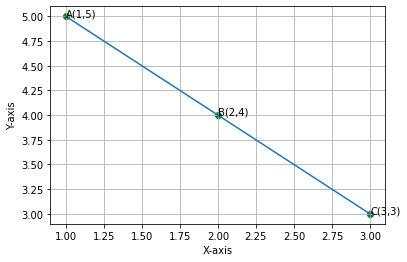
\includegraphics[width=\columnwidth]{Colinear.png}
%\caption{Line passing through points $\vec{A}$, $\vec{B}$ and $\vec{C}$}
%\label{myfig}
%\end{figure}\\
%\end{document}
